\documentclass[10pt,a4paper]{article}
\usepackage{fontspec}
\usepackage{booktabs}
\usepackage{graphicx}
\usepackage{geometry}
\usepackage{xcolor}
\usepackage{amsmath}
\usepackage[colorlinks=true,linkcolor=blue!45!black,urlcolor=blue!45!black]{hyperref}
\setmainfont{Source Han Serif CN}
\setsansfont{Source Han Sans CN}
\setmonofont{DejaVu Sans Mono}[Scale=0.9]
\XeTeXlinebreaklocale "zh"
\XeTeXlinebreakskip = 0pt plus 1pt
\geometry{margin=2.2cm}
\setlength{\parindent}{2em}
\setlength{\parskip}{0.35em}
\renewcommand{\arraystretch}{1.08}
\title{\sffamily\bfseries versor-java 性能基准报告}
\author{\sffamily 几何代数核心（纯数学，无 Minecraft 依赖）}
\date{%%DATE%%}
\begin{document}
\maketitle

\section{结论摘要}
\begin{itemize}
\item 稠密几何积是唯一的热点原语：每对 blade 约 0.78--1.06 ns，维度每增加 1 总成本约乘 4。
\item n$\ge$9 的符号表悬崖已消除：\texttt{gp} 从 40.14 ms 降到 0.916 ms（43.8$\times$）；
      Cl(10) 符号表按需构建，最多约 4 MiB。
\item E3/PGA3 快速路径：E3 旋转 16.1 ns（通用 69.7 ns），PGA 点变换 29.0 ns（通用 144.1 ns）。
\item 批量 SoA 在 N$\ge$100 时约为逐元素路径的 1.5--1.7 倍，每点分配 128 B（逐元素 169 B）。
\item JOML 单次运算快 3--13 倍；适配层是开销：motor 转 Matrix4f 约 364 ns，
      Blaze3D 每次重算矩阵约 370 ns。
\item C2 相对仅 C1 在稠密路径上快 3.07 倍；快速路径仅 1.86 倍。
\end{itemize}

\section{环境与方法}
\begin{tabular}{p{2.4cm}p{13cm}}
\toprule
CPU & %%CPU%% \\
JDK & %%JDK%% \\
JOML & %%JOMLVERSION%% \\
测量 & 单线程；校准到约 %%TARGET%%；预热 %%WARMUP%% 轮；取 %%ROUNDS%% 轮最小值 \\
\bottomrule
\end{tabular}

每个测量点自动校准迭代次数，输入用固定种子随机生成；分配量取自线程分配计数
（ThreadMXBean）。JIT 对照使用 \texttt{-XX:TieredStopAtLevel=1} 与默认 C2。
本机非隔离环境，绝对纳秒存在 $\pm$10\% 抖动，跨行比较优先看比例。未使用 JMH。

\section{维度扫描}
表 1 为稠密输入下各运算的单次耗时。图 1 与图 2 给出几何积的缩放：总时间按 $4^n$
增长，而每对 blade 的成本近似恒定。

%%SWEEP%%

\begin{figure}[htbp]\centering
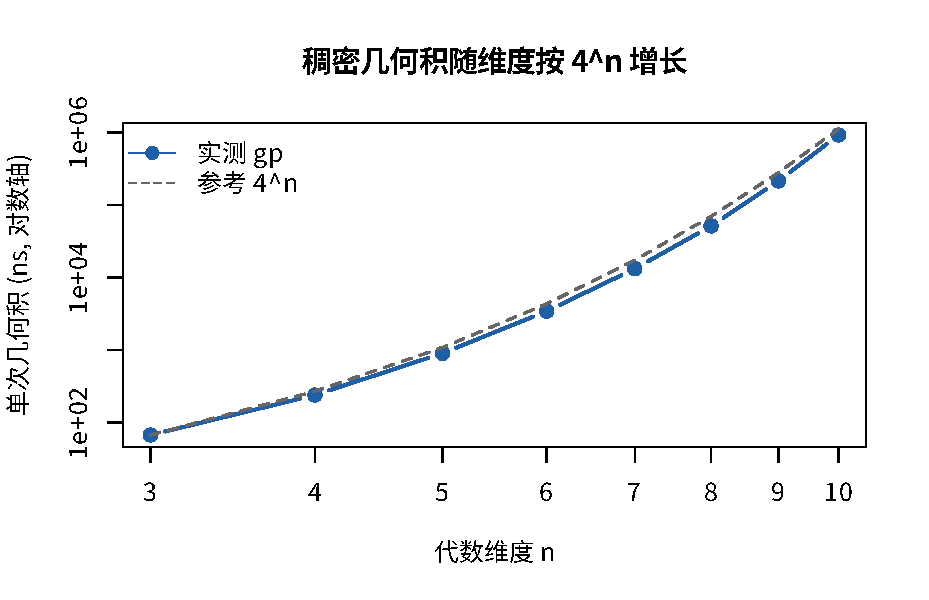
\includegraphics[width=0.82\textwidth]{figures/fig-gp.pdf}
\caption{稠密几何积随维度按 $4^n$ 增长。}\label{fig:gp}
\end{figure}

%%PAIRS%%

\begin{figure}[htbp]\centering
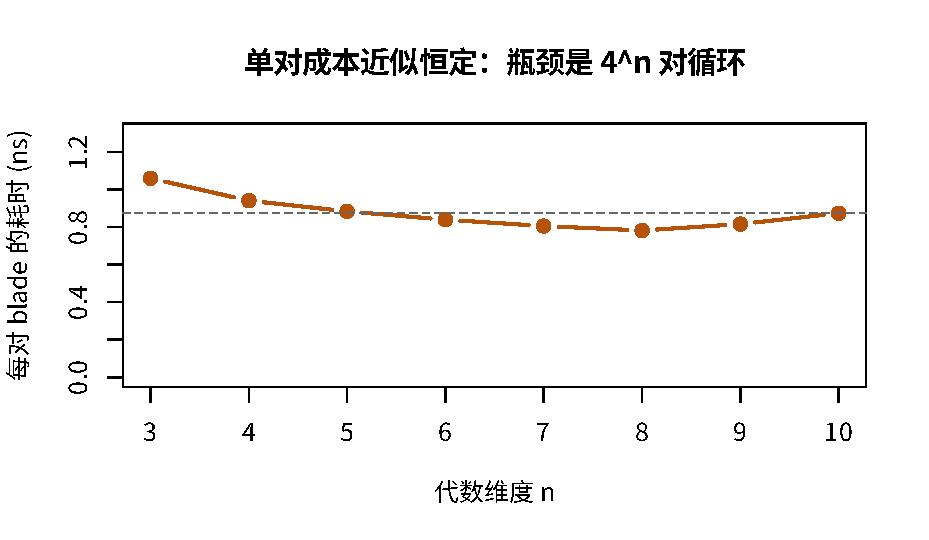
\includegraphics[width=0.82\textwidth]{figures/fig-perpair.pdf}
\caption{每对 blade 的耗时近似恒定，说明瓶颈是循环规模而非符号表查询。}\label{fig:pair}
\end{figure}

\subsection{高维符号表悬崖}
此前 n$\ge$9 没有预计算符号表，每对 blade 现场推导符号，单对成本从约 0.9 ns
升到约 36 ns。下表为修复前后的对比；现在符号表在首次乘法时按需构建。

%%CLIFF%%

\section{批量与内存布局}
\texttt{MultivectorBatch} 按 blade 连续存储（SoA），E3/PGA3 使用与标量快速路径相同的
展开公式，一次 \texttt{sandwich} 只分配结果数组。N=1 时批量有约 262 ns 固定开销，
不适合单元素；N$\ge$100 时开始超过逐元素路径。

%%BATCH%%

\begin{figure}[htbp]\centering
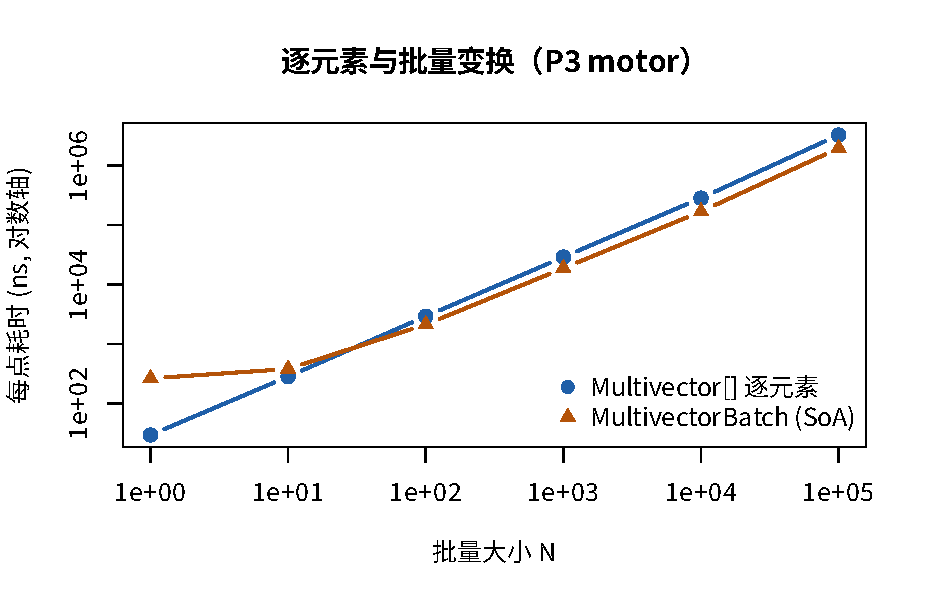
\includegraphics[width=0.82\textwidth]{figures/fig-batch.pdf}
\caption{批量与逐元素的每点成本。}\label{fig:batch}
\end{figure}

\section{快速路径与稀疏性}
%%SPARSE%%

E3 rotor$\times$vector 为 16.1 ns，通用路径 69.7 ns；PGA3 motor$\times$point 为 29.0 ns，
通用路径 144.1 ns。Cl(4) 稠密 sandwich 为 502.7 ns，稀疏 motor 输入为 129.3 ns。

\section{与 JOML 对比}
%%JOML%%

\begin{figure}[htbp]\centering
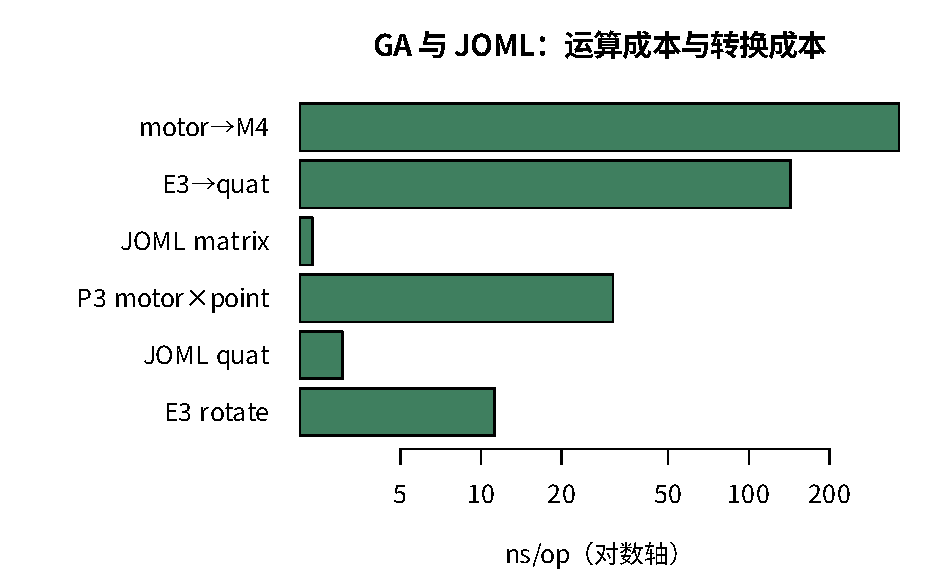
\includegraphics[width=0.9\textwidth]{figures/fig-joml.pdf}
\caption{GA 与 JOML：单次运算与转换成本。}\label{fig:joml}
\end{figure}

JOML 使用 float 且多数 API 原地写回，因此单次四元数/矩阵变换快 3--13 倍；GA 路径返回
不可变 \texttt{Multivector}，包含一次分配。真正的差异来自适配层：
\texttt{Blaze3D.matrix(motor)} 每次调用重算旋转矩阵与平移（约 364 ns），
\texttt{Blaze3D.transform} 每次重算矩阵（约 370 ns），比直接 sandwich 慢 12 倍。
渲染热路径应缓存 \texttt{Matrix4f}。float JOML 与 double GA 的坐标最大差为 3.7e-7。

\section{压力测试}
%%STRESS%%

\texttt{inverseGeneral} 随维度约 7--8 倍增长（$O(8^n)$），n=8 单次约 9.1 ms；
3$\times$3 多向量矩阵求逆稳定在约 13 $\mu$s，主要成本是 9 次通用主元求逆与消元。
这两者都只适合中小规模或一次性求解，不应进入逐帧循环。

\section{JIT 层级}
%%JIT%%

\begin{figure}[htbp]\centering
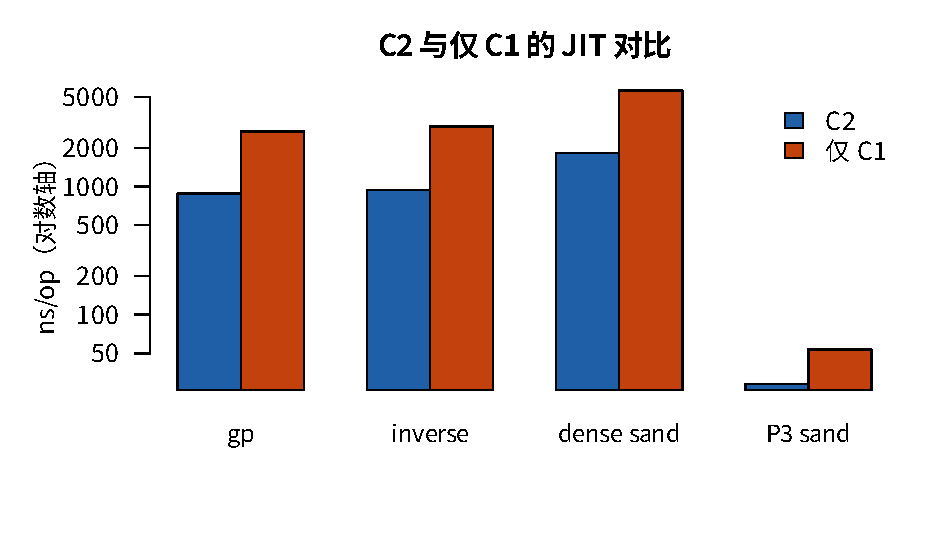
\includegraphics[width=0.82\textwidth]{figures/fig-jit.pdf}
\caption{同一基准在 C2 与仅 C1 下的对比。}\label{fig:jit}
\end{figure}

\section{建议}
\begin{enumerate}
\item 几何积的 $4^n$ 稠密循环是唯一值得继续研究的算法瓶颈；单对成本已接近常数，
      进一步提升需要稀疏/分块表示，而不是微优化。
\item 符号表按需构建已消除 n$\ge$9 的 44$\times$ 悬崖；Cl(10) 首次乘法多一次建表开销。
\item 批量 API 用于 N$\ge$100 的批量变换；单元素保持使用不可变 API。
\item 渲染侧缓存 \texttt{Matrix4f}/\texttt{Quaternionf}，避免逐调用转换。
\item \texttt{inverse()} 仅用于 versor；一般元素和矩阵主元使用
      \texttt{inverseGeneral()}，并限制维度。
\item 本报告覆盖了 ga-benchmark 的大部分一元/二元运算，但该规范没有 Java 绑定，
      因此没有直接接入；横向比较对象为 JOML。
\end{enumerate}

\section{复现}
\begin{verbatim}
cd lib/versor-java
./bench.sh                 # full suite (adds JOML when found)
./bench.sh sweep           # dimension sweep only
cd report && Rscript report.R   # rebuild PERFORMANCE.pdf
\end{verbatim}

\section{限制}
单机、单线程、非隔离环境；分配量来自 TLAB 计数，适合比较数量级；JOML 为 float，
不是同精度纯算术对比；未实现真实 SIMD（Java Vector API 仍为 incubator）。

\end{document}
